 \thispagestyle{gocconone}
\pagestyle{gocco}
\everymath{\color{gocco}}
\graphicspath{{../gocco/pic/}}
\blfootnote{$^1${\color[named]{gocco}Trung tâm Quy hoạch và Điều tra tài nguyên -- môi trường biển khu vực phía Nam.}}
\begingroup
\AddToShipoutPicture*{\put(0,616){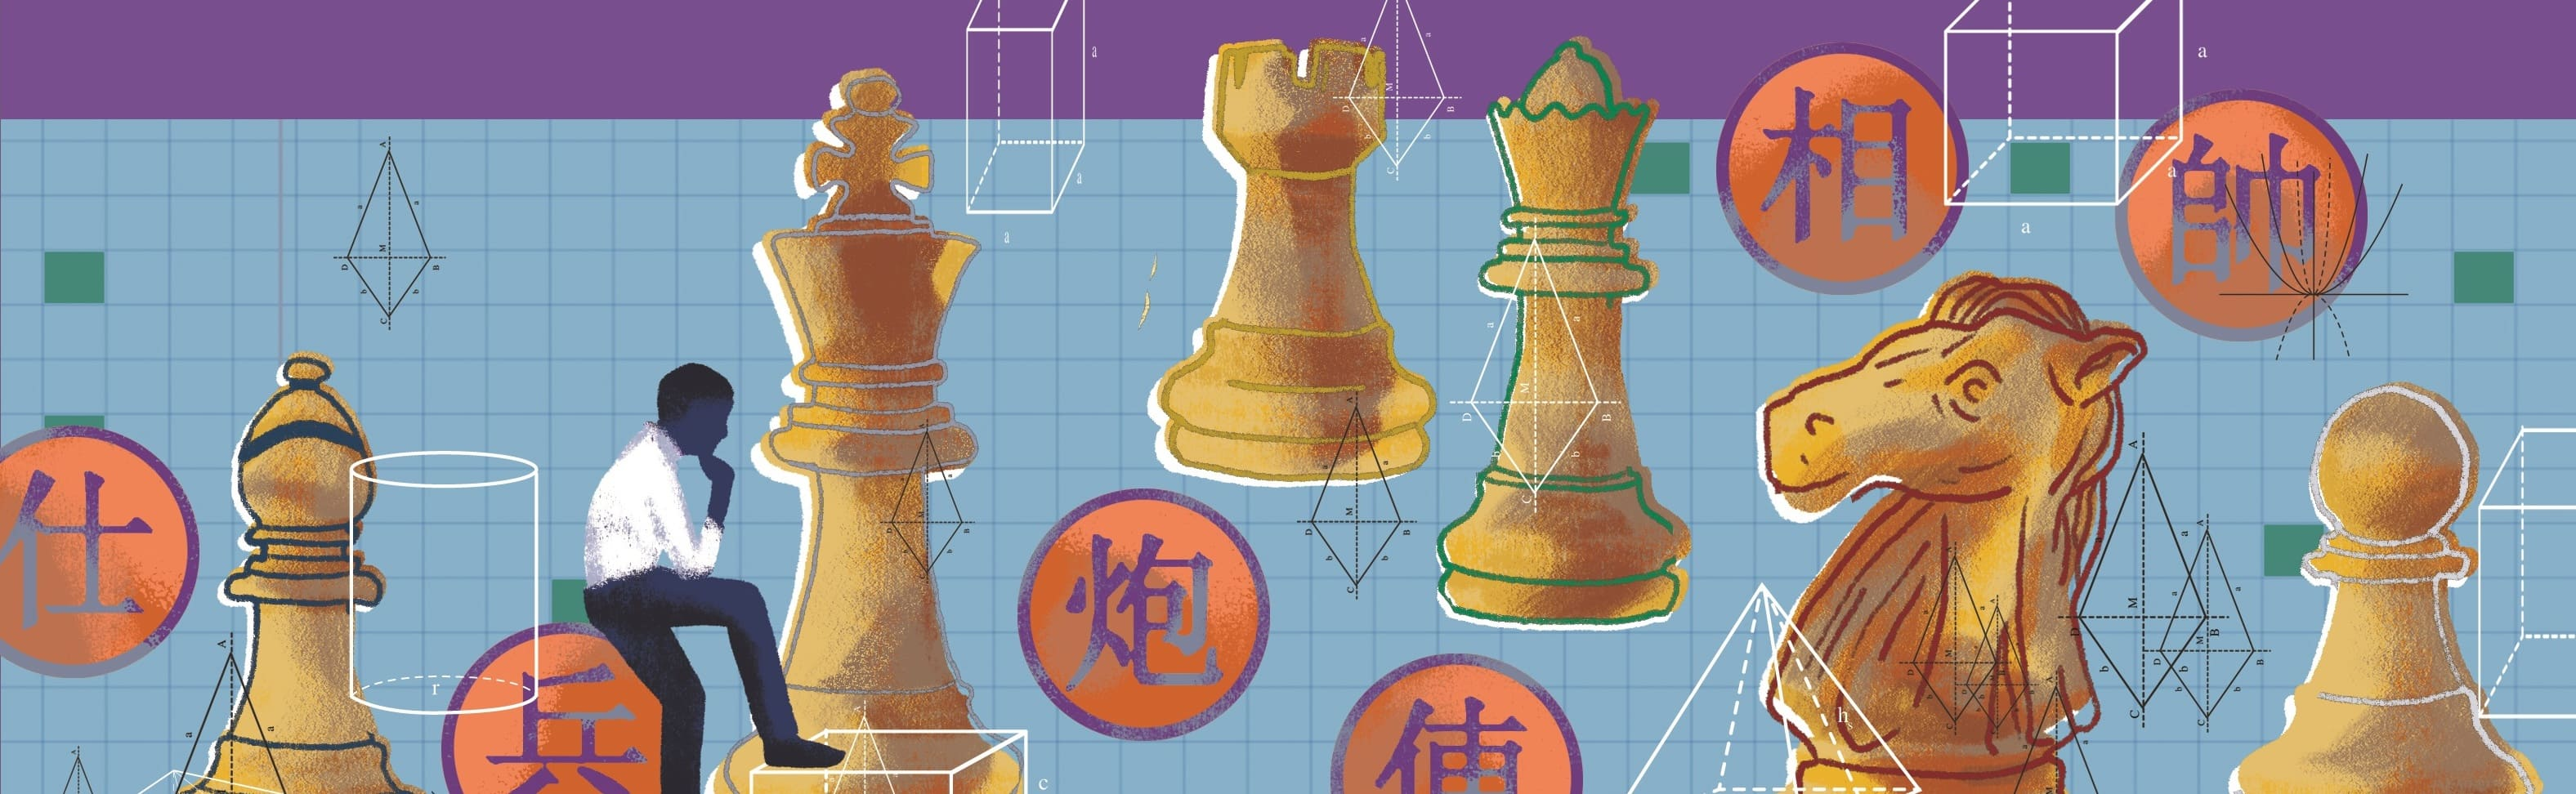
\includegraphics[width=19.3cm]{../bannergocco}}}
\AddToShipoutPicture*{\put(90,555){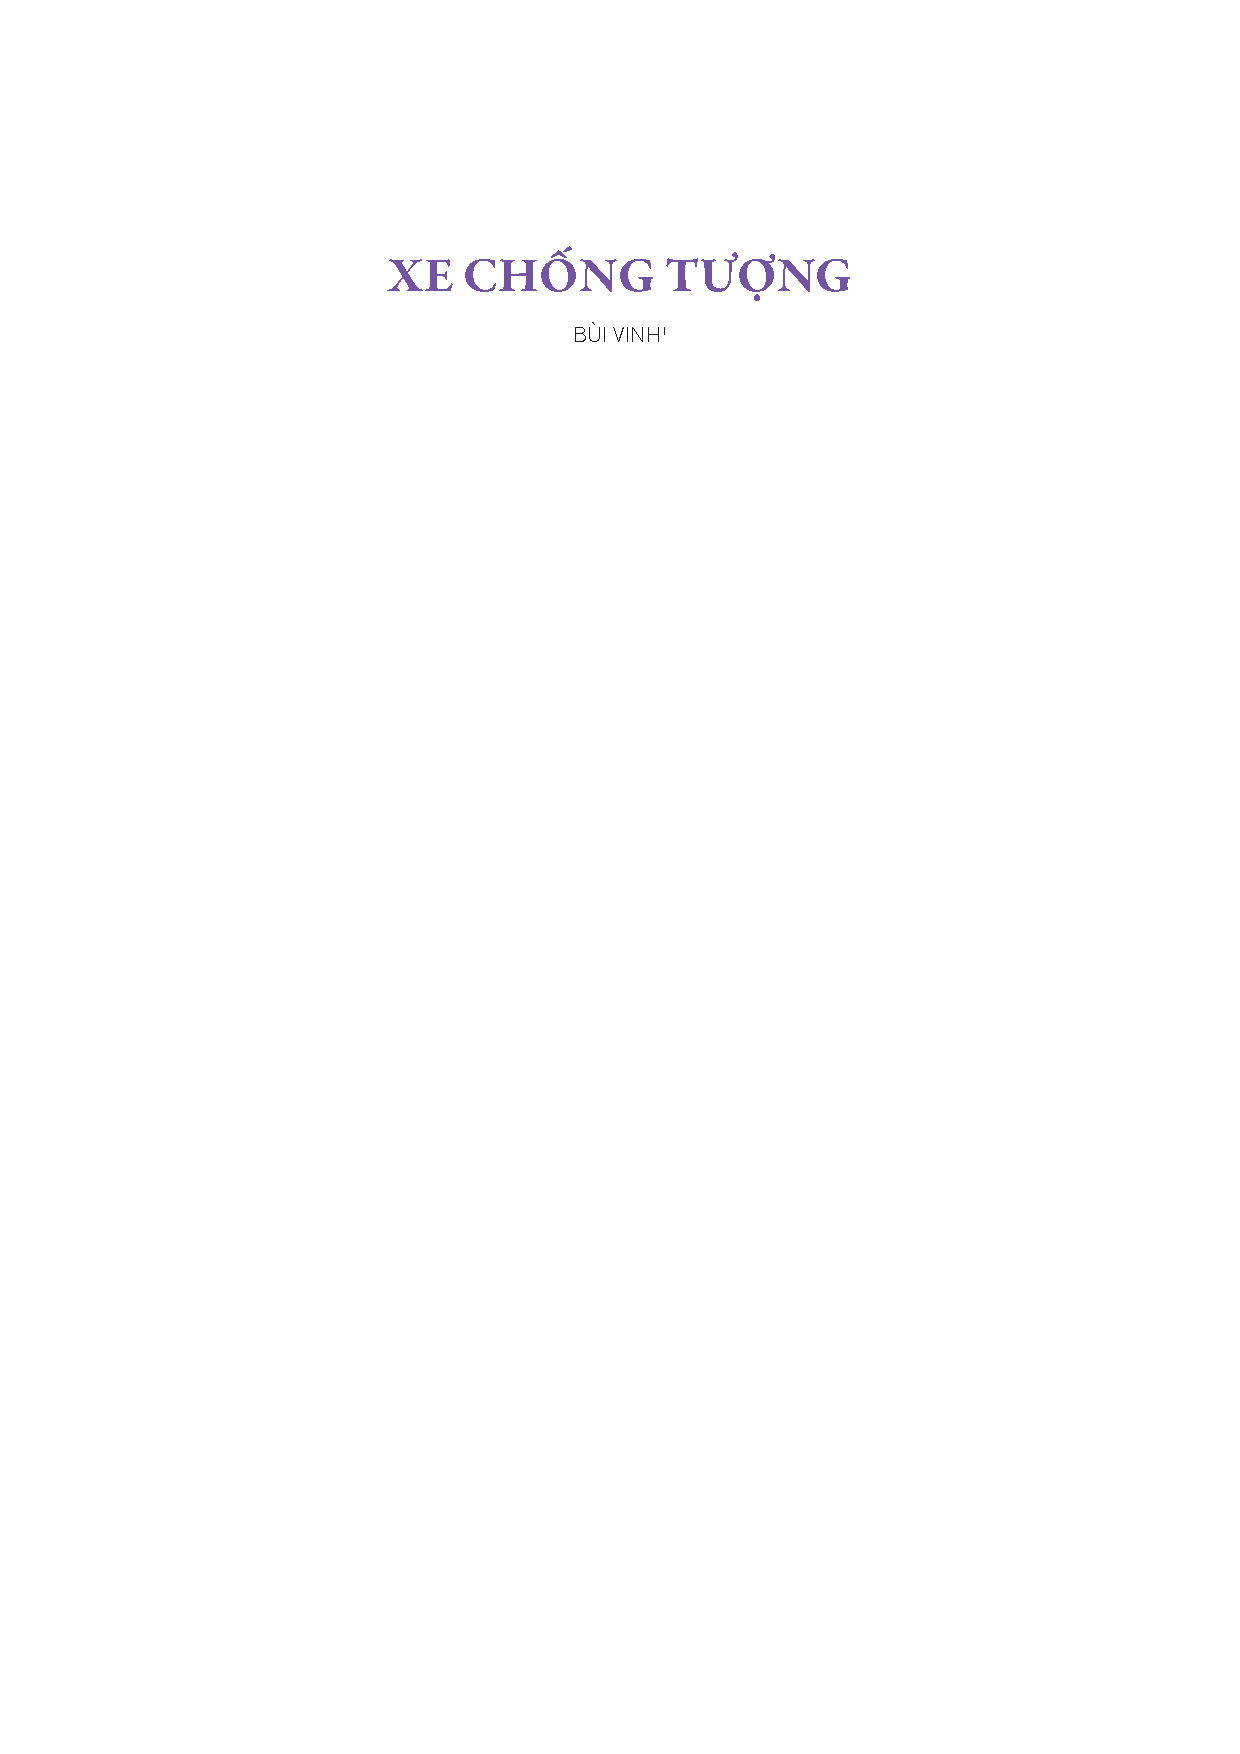
\includegraphics[scale=1]{../tieude.pdf}}} 
\centering
\endgroup

\vspace*{150pt}
\begin{multicols}{2}

%	“\textit{Xe mười, Pháo bảy, Ngựa ba}”, như một lẽ tất nhiên, Xe luôn được đánh giá là quân có sức mạnh lớn nhất trên bàn cờ, sự sống còn của Xe sẽ quyết định phần nào đến kết quả thắng bại sau cùng của mỗi cuộc chiến. Sở hữu khả năng di chuyển linh hoạt, ăn quân và khống chế tầm xa theo $2$ chiều ngang dọc, Xe luôn thể hiện tính cơ động, có thể lui tới tất cả $90$ giao điểm trên bàn cờ. Mỗi nước đi, mỗi nước tấn công của quân Xe cũng hàm chứa những ý nghĩa thâm sâu đằng sau nó. Quân Xe mang cho mình hình tượng của một người quân tử thời xưa, một trang nam nhi đầu đội trời, chân đạp đất, khí phách hiên ngang, tài giỏi, chính trực và anh hùng. Vì vậy, Xe luôn thẳng thắn đối đối diện với kẻ thù trong mọi tình huống dù là nguy hiểm nhất, luôn ra đòn tấn công trực diện, không bao giờ có ý nghĩ tập kích từ phía sau lưng.
%	\vskip 0.05cm
	Vì lẽ đó, Xe luôn chiếm một vai trò đặc biệt quan trọng trong mỗi trận chiến, bất kể đó đang là giai đoạn khai cuộc, trung cuộc hay tàn cuộc; khi đang tấn công hay khi cần lui về phòng thủ. Giai đoạn đầu mỗi ván đấu, đôi Xe luôn được ưu tiên xuất động nhanh\linebreak chóng, chiếm đóng các con đường huyết mạch, những trục lộ trọng yếu, vừa tạo điểm tựa vững chắc cho các binh chủng khác lấy đó làm bàn đạp tiến vào đất địch, và đồng thời cũng cản trở, vô hiệu hóa hướng phát triển quân của kẻ địch. Trải qua giai đoạn trung -- tàn cuộc, sau những nước đổi quân, lực lượng đôi bên càng giảm, Xe lại càng thể hiện sức mạnh với những đòn uy hiếp, dồn ép đầy uy lực, mang tính sát thương cao. Trong những tình huống cụ thể, Xe có thể phối hợp tác chiến với những quân chiến khác để tạo ra những đợt truy kích, đánh phá dồn dập khiến đối phương không kịp \linebreak phản đòn. 
	\vskip 0.1cm
	Ngoài sức tấn công mạnh mẽ, Xe còn có khả năng phòng thủ vô cùng tuyệt vời. Dù cho đang vất vả nơi chiến trường hay biên ải xa xôi, nhưng một khi cửu cung bị đe dọa, Xe có thể quay về một cách nhanh chóng để giải nguy, hộ giá kịp thời.
	Để minh chứng những điều kể trên, chúng ta hãy cùng nhau xét một vài hình cờ cụ thể:
	\begin{figure}[H]
		\vspace*{-5pt}
		\centering
		\captionsetup{labelformat= empty, justification=centering}
		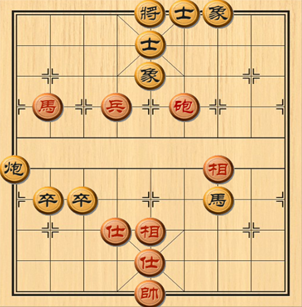
\includegraphics[width= 0.32\textwidth]{1}
		\caption{\small\textit{\color{gocco}Hình $1$.}}
		\vspace*{-10pt}
	\end{figure} 
	$1.$ Hình $1$, thoạt nhìn thì bên Đỏ đang rơi vào thế khó, Đen có Pháo giác và song Xe áp cửu rất nguy hiểm, chỉ cần đi X$3-5$ hoặc X$7-5$ là tạo nên sát cục. Nhưng bên Đỏ được quyền đi trước, Đỏ ra đòn như sau:
	\vskip 0.05cm
	$\pmb{1)}$ X$9.6$   S$5/4$\quad $\pmb{2)}$ X$9-6^*$ Tg$-4$\quad $\pmb{3)}$ X$4.9^{**}$ Tg$.1$\quad $\pmb{4)}$ X$4-5^{***}$ X$3-6$\quad $\pmb{5)}$ M$8.7$ $(1-0)$
	\vskip 0.05cm
	\textit{$*$: $2$ nước tấn Xe rồi phế Xe vào Sĩ đầy uy lực, ép Tướng Đen phải ra khỏi vị trí an toàn, từ lúc này Đỏ bắt đầu mở ra một đợt phản công  dồn dập về phía đối phương.
		\vskip 0.05cm
		$**$: Tiếp tục là nước di chuyển Xe rất hay, vừa tấn lên phá Sĩ tạo áp lực cho Tướng địch, vừa chừa lộ cho Tướng Đỏ có thể thoát hiểm trong tương lai.
		\vskip 0.05cm
		$***$: Nước bình Xe nhẹ nhàng nhưng đầy sát khí, chỉ cần nhảy Mã tới là hết cờ, Đen dù cố gắng bình Xe dọa chém Sĩ tạo sát nhưng vẫn chậm hơn $1$ nhịp, đành chấp nhận thất bại.}
	\begin{figure}[H]
		\vspace*{-5pt}
		\centering
		\captionsetup{labelformat= empty, justification=centering}
		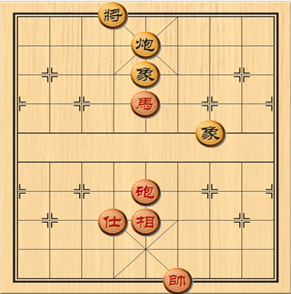
\includegraphics[width= 0.32\textwidth]{2}
		\caption{\small\textit{\color{gocco}Hình $2$.}}
		\vspace*{-10pt}
	\end{figure}
	$2.$ Hình $2$, bên Đen dường như nắm lợi thế lớn vì $4$ quân: Xe, Pháo, Mã, Chốt đang ở vị trí đắc địa, mặc dù Đỏ còn song Xe nhưng thế công không rõ ràng, lại còn khuyết Sĩ, Tượng. Cứ ngỡ Đen chỉ cần X$3.2$ là giành\linebreak chiến thắng. Nhưng không, Đỏ được đi trước và có những nước đi vô cùng khéo léo:
	\vskip 0.05cm
	$\pmb{1)}$ X$2-7^*$ X$3-8^{**}$ \quad$\pmb{2)}$ X$7-3^{***}$ T$7.9$\quad $\pmb{3)}$ P$2.5^{****}$ X$9-6$\quad $\pmb{4)}$ X$4/6$ $(1-0)$
	\vskip 0.05cm  
	\textit{$*$: Nước bình Xe đầy bất ngờ và tinh tế, vừa mở đường cho Pháo Đỏ lao xuống tấn công, vừa ngăn chặn ý đồ tấn Xe tạo sát của Đen. Nếu Đen vô tư chơi X$3/4$ ăn Xe thì Đỏ cắm Pháo đáy tạo sát cục, lúc này dù Đen có lên Tượng hay về Sĩ cũng đều thất bại.
		\vskip 0.05cm
		$**$: Nước đi bắt buộc của Đen, vừa tránh mất Xe, vừa phá hỏng ý đồ chơi P$2.6$ của bên Đỏ.
		\vskip 0.05cm
		$***$: Với sự cơ động của chiến Xe, Đỏ lại tiếp tục bình sang bắt Tượng, chuẩn bị cho đòn Song Xe tạo sát.
		\vskip 0.05cm
		$****$: Với nước tấn Pháo cản eo Tượng nhẹ nhàng này, Đỏ vẫn không từ bỏ ý định đi X$3.2$ bắt sống tướng giặc. Đen không còn lựa chọn nào hay hơn, đành chấp nhận bỏ Xe để hộ giá. Đen không còn Xe, chiến thắng cho Đỏ chỉ còn là vấn đề thời gian.}
	\begin{figure}[H]
		\vspace*{-5pt}
		\centering
		\captionsetup{labelformat= empty, justification=centering}
		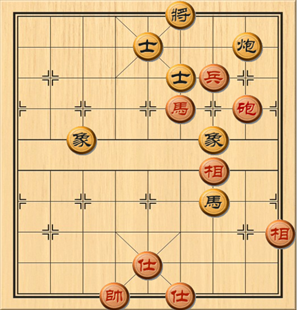
\includegraphics[width= 0.32\textwidth]{3}
		\caption{\small\textit{\color{gocco}Hình $3$.}}
		\vspace*{-10pt}
	\end{figure}
	$3.$ Hình $3$, Đen đang tạo áp lực lên trận địa bên đỏ với $3$ quân: Xe, Pháo, Chốt tham chiến. Tuy nhiên, Đỏ đang có Pháo kiềm chế Xe, Sĩ bên Đen tại trục lộ $6$ và được quyền đi trước, Đỏ ra đòn như sau:
	\vskip 0.05cm
	$\pmb{1)}$ X$4.7$ Tg$.1$\quad $\pmb{2)}$ X$4/2$ Tg$-5$\quad $\pmb{3)}$ X$4-5$ Tg$-4$\quad  $\pmb{4)}$ X$5-6^*$ Tg$-5$\quad $\pmb{5)}$ P$6-5$ $(1-0)$
	\vskip 0.05cm
	\textit{$*$: Tranh thủ nước tiên và sự cơ động của Xe, Đỏ liên tiếp có những nước đi vô cùng hiệu quả, hết chiếu tướng, thoái bắt Sĩ, nhảy Xe thẳng vào nơi nguy hiểm rồi lại đánh Sĩ. Sau mỗi nước di chuyển Xe của Đỏ, Đen phải vất vả di chuyển Tướng để giải nguy.}
	\vskip 0.05cm
		\textit{$**$: Sau khi điều được chiến chiến Xe chiếm được trục lộ trọng yếu, Đỏ nhẹ nhàng bình Pháo kết liễu đối phương.}
		\vskip 0.05cm
		\textbf{\color{gocco}Câu đố kỳ này}
		\vskip 0.05cm
		Đỏ sẽ tận dụng nước tiên và vận dụng những đòn phối hợp Xe và các binh chủng khác như thế nào để giành chiến thắng trong các hình cờ dưới đây?
		\begin{figure}[H]
					\vspace*{-5pt}
					\centering
					\captionsetup{labelformat= empty, justification=centering}
					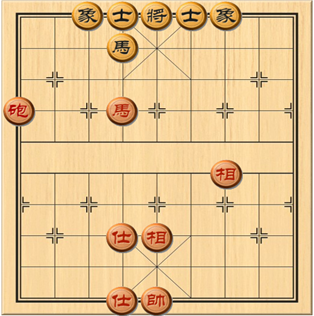
\includegraphics[width= 0.32\textwidth]{4}
					\caption{\small\textit{\color{gocco}Hình $4$.}}
					\vspace*{-10pt}
				\end{figure}
	%	\textit{Đáp án tham khảo:} $\pmb{1)}$ X$8-6$ Tg$.1$\quad $\pmb{2)}$ M$2/4$ Tg$.1$ \quad$\pmb{3)}$ M$4.5$ Tg$/1$\quad $\pmb{4)}$ X$2.8$ Tg$/1$ \quad $\pmb{5)}$ P$4-7$ $(1-0)$
		\begin{figure}[H]
					\vspace*{5pt}
					\centering
					\captionsetup{labelformat= empty, justification=centering}
					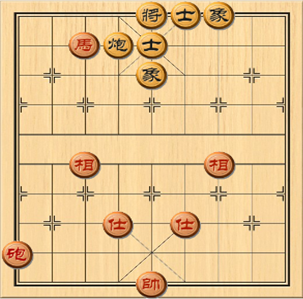
\includegraphics[width= 0.32\textwidth]{5}
					\caption{\small\textit{\color{gocco}Hình $5$.}}
					\vspace*{-10pt}
				\end{figure}
	%	\textit{Đáp án tham khảo:} $\pmb{1)}$ X$4.5$ Tg$.1$ \quad $\pmb{2)}$ X$4/1$ Tg$/1$\quad $\pmb{3)}$ X$5.1$ S$4.5$\quad $\pmb{4)}$ X$5.1$ Tg$-4$\quad $\pmb{5)}$ X$4.1$ $(1-0)$
		\vskip 0.05cm   
		\textit{Chú thích: C: Chốt, X: Xe, M: Mã, P: Pháo, Tg: Tướng, S: Sĩ, T: Tượng.}
\end{multicols}




